\documentclass[authoryear,preprint,12pt]{elsarticle}

\usepackage{amsmath,amssymb,amsfonts}
\usepackage{lmodern}
\usepackage{graphicx}
\usepackage{booktabs}
\usepackage{tabularx}
\usepackage{multirow}
\usepackage{lineno}
\usepackage{hyperref}
\usepackage{microtype}
\usepackage{adjustbox}
\usepackage[margin=2.5cm]{geometry}

\journal{Chemosphere}

\begin{document}

\begin{frontmatter}

\title{Dissolved and Unspecified-Fraction Heavy Metals in Bangladesh River Waters: A Synthesis of Published Records (2010--2022), Benchmark Exceedances, and Seasonal Contrasts}

\author[inst1]{Author One\corref{cor1}}
\ead{author.one@university.edu}
\author[inst1,inst2]{Author Two}
\ead{author.two@institution.org}
\author[inst2]{Author Three}
\ead{author.three@research.org}

\cortext[cor1]{Corresponding author. Tel.: +880-XXXXXXXXXX.}

\affiliation[inst1]{organization={Department of Environmental Science and Engineering},
            addressline={University Name}, 
            city={Dhaka},
            postcode={1000},
            country={Bangladesh}}

\affiliation[inst2]{organization={Institute of Water and Flood Management},
            addressline={Technical University}, 
            city={Dhaka},
            postcode={1205},
            country={Bangladesh}}

\begin{abstract}
River water in the Bengal Delta provides indispensable freshwater for regional ecology, agriculture, and municipal water abstraction, but rivers receive substantial industrial and municipal effluent loadings. Here, we present a systematic multi-study synthesis of heavy metal concentrations in Bangladesh river waters by compiling an audited literature database of 268 records across 12 major river systems from 28 peer-reviewed field investigations (2010--2022). Concentrations were evaluated against international health reference benchmarks (WHO Guidelines for Drinking-water Quality, 4th ed.\ incorporating 2022 addenda) and statutory domestic standards (Bangladesh Environmental Conservation Rules, ECR 2023 potable schedule). Substantial benchmark exceedances were documented for key toxic elements in published records: Lead (Pb) exceeded the WHO guideline (0.010~mg/L) in \textbf{85.6\%} of records (95\% Wilson CI: 79.0--90.4\%, median: 0.0286~mg/L, max: 0.700~mg/L), and exceeded the Bangladesh standard (0.050~mg/L) in \textbf{34.9\%} of records (95\% CI: 27.7--43.0\%). Exceedances of WHO benchmarks were also pronounced for total Chromium (60.6\% [52.9--67.9\%]), Nickel (54.8\% [45.2--64.0\%]), Arsenic (54.9\% [46.1--63.5\%]), and Cadmium (44.7\% [36.5--53.2\%]). A sensitivity analysis excluding capital-adjacent industrial rivers (Buriganga, Turag, Shitalakhya) showed lower national exceedances (e.g., Bangladesh standard exceedance for Pb dropped to 18.3\%, and Arsenic to 8.9\%), confirming heavy geographical clustering in the literature. Integrated Heavy Metal Pollution Index ($\mathrm{HPI}$) evaluation across multi-metal records yielded a median of 202.3 (IQR: 79.0--793.9, mean: 718.7), with 63.1\% exceeding the critical threshold of 100. Two-sided Mann-Whitney U hypothesis testing with Holm-Bonferroni family-wise adjustment confirmed statistically significant seasonal dilution for Arsenic (dry median 0.0073~mg/L vs.\ wet median 0.0042~mg/L; 1.74$\times$ ratio, $p = 0.0039$, $p_{\mathrm{adj}} = 0.027$). Chromium (2.01$\times$, unadjusted $p=0.028$) and Cadmium (1.88$\times$, unadjusted $p=0.043$) exhibited elevated dry-season medians but did not maintain significance after Holm adjustment ($p_{\mathrm{adj}} > 0.15$), while Lead showed no seasonal contrast ($p=0.854$). Geodesic reach analysis across HydroSHEDS HydroRIVERS demonstrated that 89.8\% of major national river length (9,915.9~km across 4,389 reaches) is located $>25$~km from any published sampling point, highlighting surveillance gaps in the mainstems of the Lower Meghna, Padma, and Jamuna rivers.
\end{abstract}

\begin{graphicalabstract}
\centering
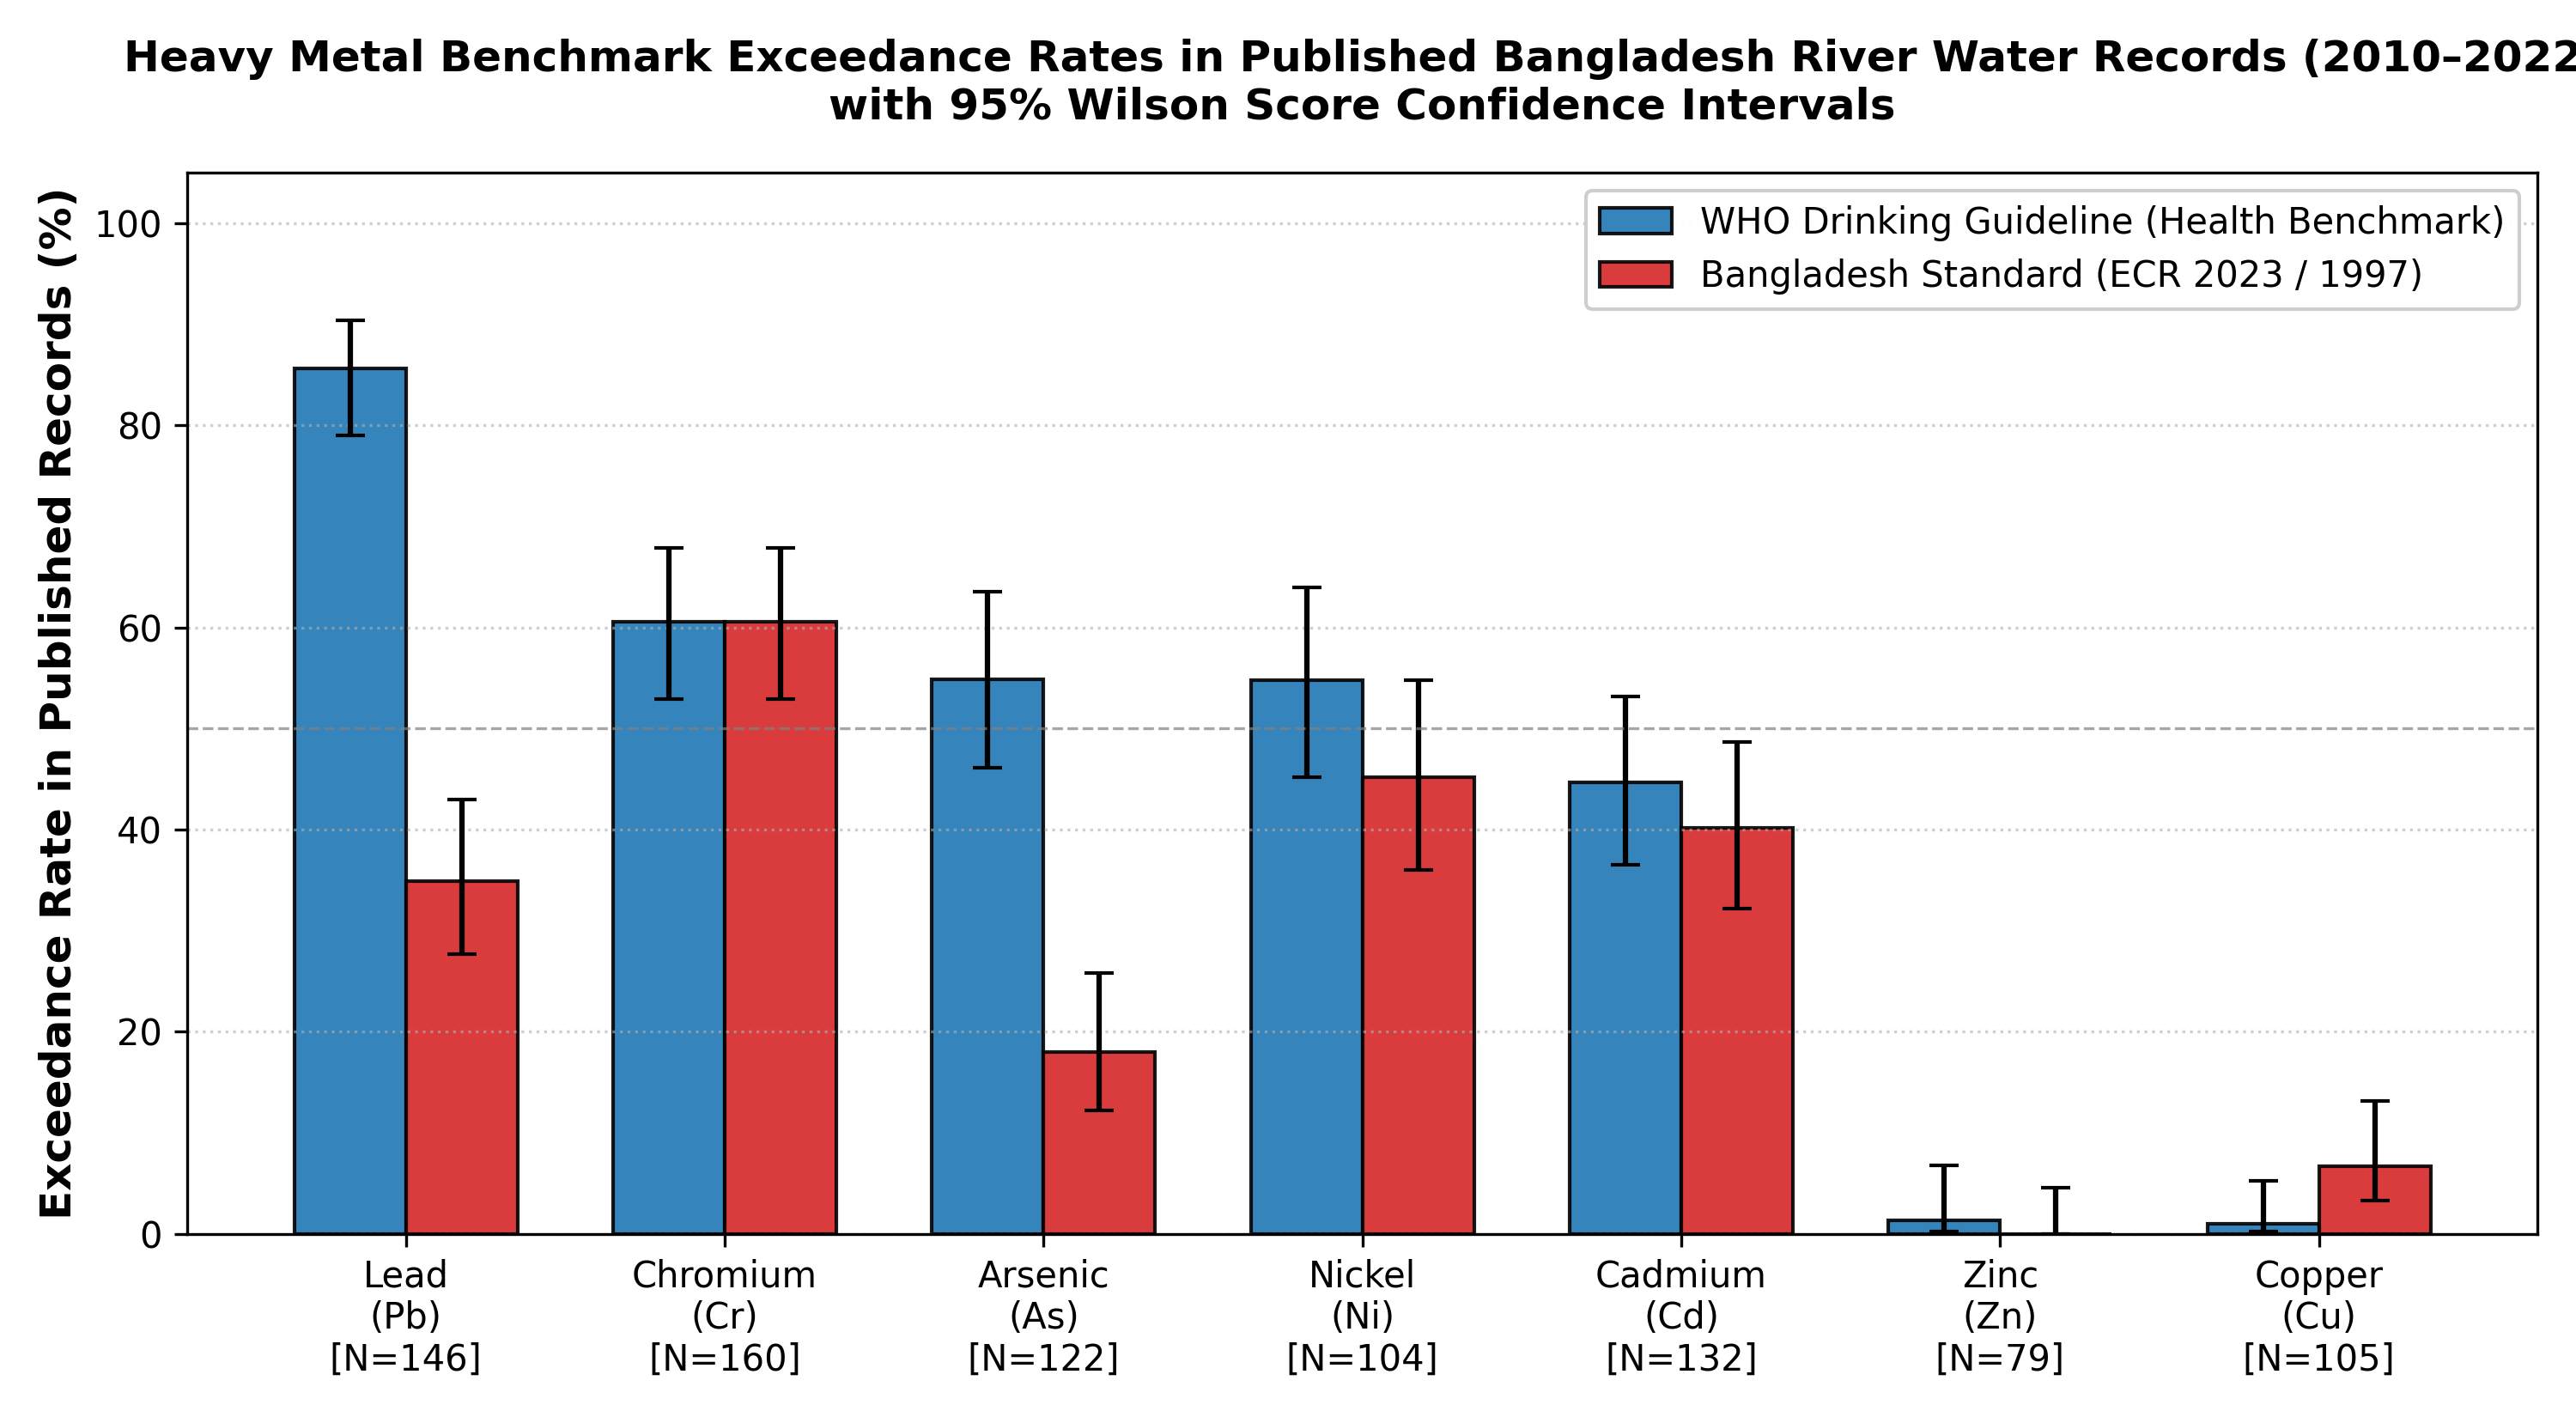
\includegraphics[width=0.85\textwidth]{fig1_exceedance.png}
\end{graphicalabstract}

\begin{highlights}
\item Synthesized 268 published heavy metal records across 12 Bangladesh rivers.
\item 85.6\% of records exceed the WHO drinking benchmark for Lead (0.01 mg/L).
\item Total Cr, Ni, and As exceed WHO guidelines in 55--61\% of published records.
\item Two-sided testing confirms seasonal dilution for Arsenic (1.74x, p\_adj = 0.027).
\item Over 89\% of major river reach length lacks published water quality monitoring.
\end{highlights}

\begin{keyword}
River water \sep Heavy metals \sep Drinking water benchmarks \sep WHO guidelines \sep Heavy Metal Pollution Index ($\mathrm{HPI}$) \sep Seasonal contrast \sep Spatial surveillance gaps
\end{keyword}

\end{frontmatter}

\linenumbers

\section{Introduction}
Surface freshwater networks formed by the Ganges, Brahmaputra, and Meghna (GBM) river basins support over 170 million people in Bangladesh, sustaining irrigated agriculture, capture fisheries, municipal intake facilities, and industrial supply \citep{Ahmad2010,Datta1998}. However, rapid industrial growth across the textile dyeing, leather tanning, pharmaceutical, and chemical manufacturing sectors, combined with untreated municipal discharges, has introduced significant toxic contaminants into fluvial corridors \citep{Bhuiyan2015,Islam2015}.

Among aquatic pollutants, heavy metals and metalloids (e.g., As, Cd, Cr, Cu, Ni, Pb, Zn) present persistent environmental health concerns because of their non-biodegradability and potential for bioaccumulation \citep{Jarup2003,Tchounwou2012}. Chronic ingestion or exposure to elevated trace element levels can cause nephrotoxicity, neurodevelopmental deficits, and cardiovascular diseases \citep{Needleman2004,Saha2017}. To protect public health, the World Health Organization \citep{WHO2022} and the Department of Environment (DoE), Bangladesh \citep{ECR2023} have established concentration benchmarks. While untreated surface river water is not tap water delivered at the point of consumption, comparing raw river concentrations against potable water benchmarks provides a conservative screening index of environmental degradation and source-water stress \citep{Li2018}.

Evaluating published data on heavy metals in Bangladeshi river waters involves several methodological complexities. First, published literature is predominantly concentrated in heavily industrialized, capital-adjacent river reaches (e.g., Buriganga, Turag, and Shitalakhya), potentially creating geographic selection bias if literature-derived metrics are interpreted as national baseline prevalence \citep{Hossain2021}. Second, Bangladesh experiences strong hydrological seasonality, with peak South Asian monsoon precipitation between June and October contrasting sharply with dry-season low flows between November and March. Discharge-driven hydraulic dilution has been hypothesized to lower dissolved concentrations during wet periods, but multi-element statistical evaluations using rigorous multiplicity corrections remain limited. Third, spatial coverage across the national river network has not been quantified relative to established hydrological datasets, leaving the extent of geographical monitoring blind spots uncharacterized.

To address these questions, this study presents a descriptive synthesis of published river water records (2010--2022) across Bangladesh to:
\begin{enumerate}
    \item Screen trace element concentrations against WHO reference guidelines and Bangladesh statutory standards, incorporating 95\% Wilson score confidence intervals and sensitivity analyses excluding urban industrial hotspots.
    \item Evaluate multi-metal water pollution status using the Heavy Metal Pollution Index ($\mathrm{HPI}$), Heavy Metal Evaluation Index ($\mathrm{HEI}$), and Metal Index ($\mathrm{MI}$).
    \item Statistically evaluate dry-versus-wet seasonal contrasts using two-sided non-parametric hypothesis testing with Holm-Bonferroni family-wise error rate corrections.
    \item Quantify the spatial coverage of published monitoring stations along major river reaches using geodesic distance routing in HydroSHEDS HydroRIVERS.
\end{enumerate}

\section{Materials and Methods}

\subsection{Literature Compilation and Quality Screening}
An audited literature compilation was conducted across peer-reviewed investigations published between 2010 and 2022 reporting heavy metal concentrations in Bangladesh river waters \citep{Ahmad2010,Ali2016,Ali2021,Bhuiyan2015,Hossain2021,Islam2015,Kadir2022,Mortuza2024}. Original source tables and analytical methods were audited to standardize concentration units into milligrams per liter ($\text{mg/L}$) and micrograms per liter ($\mu\text{g/L}$). Extreme values and candidate outliers were audited against primary publication texts, verifying reporting units and instrument calibrations. In total, 268 surface water records across 12 river systems (Buriganga, Turag, Shitalakhya, Karnaphuli, Korotoa, Padma, Meghna, Surma, Kirtankhola, Rupsa, Paira, and Old Brahmaputra) were assembled into a structured database.

Because several primary publications did not explicitly document membrane filtration protocols (e.g., 0.45~$\mu\text{m}$ pre-filtration versus total digestion), measurements are treated conservatively as dissolved or unspecified-fraction concentrations. Seven trace elements with adequate multi-study representation were analyzed: As ($N=122$), Cd ($N=132$), Cr ($N=160$), Cu ($N=105$), Ni ($N=104$), Pb ($N=146$), and Zn ($N=79$).

\subsection{Water Quality Reference Benchmarks and Statistical Intervals}
Observed concentrations were compared against established reference frameworks:
\begin{enumerate}
    \item \textbf{World Health Organization \citep{WHO2022}:} Health-based guideline values for drinking-water quality: As (0.010~mg/L), Cd (0.003~mg/L), total Cr (0.050~mg/L), Cu (2.000~mg/L), Ni (0.070~mg/L), and Pb (0.010~mg/L). For Zinc, the WHO guideline value of 3.000~mg/L is an aesthetic and consumer acceptability threshold rather than a health-derived limit.
    \item \textbf{Bangladesh Environmental Conservation Rules \citep{ECR2023}:} Schedule 3 potable water standards: As (0.050~mg/L), Cd (0.005~mg/L), Cr (0.050~mg/L), Cu (1.000~mg/L), Ni (0.100~mg/L), Pb (0.050~mg/L), and Zn (5.000~mg/L).
\end{enumerate}

Benchmark exceedance proportions were quantified as the percentage of published records exceeding benchmark thresholds. Because environmental proportion estimates depend on sample size, 95\% confidence intervals were computed using the Wilson score method with continuity adjustment \citep{Wilson1927}:
\begin{equation}
\mathrm{CI}_{95\%} = \frac{\hat{p} + \frac{z^2}{2N} \pm z\sqrt{\frac{\hat{p}(1-\hat{p})}{N} + \frac{z^2}{4N^2}}}{1 + \frac{z^2}{N}}
\end{equation}
where $\hat{p}$ is the sample exceedance proportion, $N$ is the number of observations, and $z = 1.96$. To address selection bias associated with industrial clustering, sensitivity analyses were performed excluding the peri-urban rivers of Greater Dhaka (Buriganga, Turag, and Shitalakhya).

\subsection{Integrated Multi-Metal Pollution Indices}
To evaluate composite metal loadings in records where multiple elements were simultaneously determined ($N=157$, records with $\ge 3$ analyzed metals), three pollution indices were computed:
\begin{enumerate}
    \item \textbf{Heavy Metal Pollution Index ($\mathrm{HPI}$):}
    \begin{equation}
    \mathrm{HPI} = \frac{\sum_{i=1}^n W_i Q_i}{\sum_{i=1}^n W_i}
    \end{equation}
    where $W_i = \frac{1}{S_i}$ is the unit weight inversely proportional to the WHO guideline limit $S_i$, and $Q_i = \frac{M_i}{S_i} \times 100$ is the sub-index of metal $i$ with measured concentration $M_i$ \citep{Mohan1996,Prasad2001}. Standard classification criteria define $\mathrm{HPI} < 100$ as low pollution, $100 \le \mathrm{HPI} \le 200$ as moderate pollution, and $\mathrm{HPI} > 200$ as critical contamination. Because means of environmental indices can be skewed by extreme values, both medians with interquartile ranges (IQR) and means are reported.
    \item \textbf{Heavy Metal Evaluation Index ($\mathrm{HEI}$):}
    \begin{equation}
    \mathrm{HEI} = \sum_{i=1}^n \frac{H_c}{H_{\mathrm{mac}}}
    \end{equation}
    where $H_c$ is the measured concentration and $H_{\mathrm{mac}}$ is the maximum admissible concentration from WHO guidelines \citep{Edet2002}. Thresholds are: $< 10$ (low), $10\text{--}20$ (medium), and $> 20$ (high risk).
    \item \textbf{Metal Index ($\mathrm{MI}$):}
    \begin{equation}
    \mathrm{MI} = \sum_{i=1}^n \frac{C_i}{(\mathrm{MAC})_i}
    \end{equation}
    evaluated against Bangladesh statutory standards \citep{Tamasi2004}.
\end{enumerate}

\subsection{Evaluation of Seasonal Contrasts}
Sampling records were stratified into two primary hydrological seasons based on sampling months:
\begin{itemize}
    \item \textbf{Dry/Winter Season:} November to March (characterized by low river discharge and minimal baseflow).
    \item \textbf{Wet/Rainy Season:} June to October (peak South Asian monsoon precipitation and high discharge).
\end{itemize}

Given right-skewed concentration distributions, seasonal median differences were evaluated using the two-sided non-parametric \textbf{Mann-Whitney U test}. The dry-to-wet concentration ratio was quantified as:
\begin{equation}
\mathrm{Ratio} = \frac{\mathrm{Median}_{\mathrm{Dry}}}{\mathrm{Median}_{\mathrm{Wet}}}
\end{equation}
To control the family-wise error rate across seven simultaneous hypothesis tests, $p$-values were adjusted using the sequential \textbf{Holm-Bonferroni procedure} \citep{Holm1979}:
\begin{equation}
p_{\mathrm{adj}(k)} = \min\left(1, \, \max_{j \le k} \left[(m - j + 1) \, p_{(j)}\right]\right)
\end{equation}
where $p_{(1)} \le \dots \le p_{(m)}$ are ordered unadjusted $p$-values, and $m=7$.

\subsection{Spatial Coverage Analysis Across River Networks}
To quantify geographic representation and surveillance blind spots, spatial network analysis was conducted using the HydroSHEDS HydroRIVERS hydrographic dataset \citep{Lehner2013}:
\begin{enumerate}
    \item Major river channels strictly within the national borders of Bangladesh were identified: Strahler stream order $\ge 4$ and mean annual discharge $Q \ge 50\text{ m}^3/\text{s}$ (3,894 reach segments totaling 8,369.5~km).
    \item Great-circle geodesic distances from each major river reach polyline centroid to the nearest documented published sampling location were calculated using the Haversine formula to eliminate map projection distortion.
    \item Reaches situated $>10$, $>25$, and $>50$~km away from any published study were quantified in reach counts and river lengths (km).
    \item A prioritized candidate list of 15 surveillance reaches was selected based on upstream drainage area and mean discharge, enforcing a minimum spatial dispersion of $\ge 30$~km to avoid spatial autocorrelation and geographic redundancy.
\end{enumerate}

\section{Results}

\subsection{Benchmark Exceedance Synthesis}
Trace element concentrations in published Bangladesh river water records show substantial exceedances of both international and domestic drinking benchmarks (Table~\ref{tab:exceedance}, Fig.~\ref{fig:exceedance}).

\begin{table}[htbp]
\centering
\small
\caption{Benchmark exceedance evaluation of heavy metals in published Bangladesh river waters (2010--2022) against WHO guidelines and Bangladesh standards, with 95\% Wilson score confidence intervals.}
\label{tab:exceedance}
\begin{adjustbox}{width=\textwidth,center}
\begin{tabular}{lcccccccc}
\toprule
Element & $N$ & Mean (mg/L) & Median (mg/L) & Max (mg/L) & WHO Limit & WHO Exceed (95\% CI) & BD Limit & BD Exceed (95\% CI) \\
\midrule
\textbf{Lead (Pb)} & 146 & 0.0818 & 0.0286 & 0.7000 & 0.010 & \textbf{85.6\%} [79.0--90.4\%] & 0.050 & \textbf{34.9\%} [27.7--43.0\%] \\
\textbf{Chromium (Cr)} & 160 & 0.3131 & 0.0710 & 7.5500 & 0.050 & \textbf{60.6\%} [52.9--67.9\%] & 0.050 & \textbf{60.6\%} [52.9--67.9\%] \\
\textbf{Arsenic (As)} & 122 & 0.0351 & 0.0152 & 0.3520 & 0.010 & \textbf{54.9\%} [46.1--63.5\%] & 0.050 & \textbf{18.0\%} [12.2--25.8\%] \\
\textbf{Nickel (Ni)} & 104 & 0.3467 & 0.0888 & 2.8880 & 0.070 & \textbf{54.8\%} [45.2--64.0\%] & 0.100 & \textbf{45.2\%} [36.0--54.8\%] \\
\textbf{Cadmium (Cd)} & 132 & 0.0130 & 0.0028 & 0.1230 & 0.003 & \textbf{44.7\%} [36.5--53.2\%] & 0.005 & \textbf{40.2\%} [32.2--48.7\%] \\
\textbf{Zinc (Zn)} & 79 & 0.5768 & 0.4000 & 3.2000 & 3.000$^*$ & \textbf{1.3\%} [0.2--6.8\%] & 5.000 & \textbf{0.0\%} [0.0--4.6\%] \\
\textbf{Copper (Cu)} & 105 & 0.2648 & 0.0888 & 2.1790 & 2.000 & \textbf{1.0\%} [0.2--5.2\%] & 1.000 & \textbf{6.7\%} [3.3--13.1\%] \\
\bottomrule
\multicolumn{9}{l}{\footnotesize $^*$WHO guideline for Zinc (3.0 mg/L) is based on aesthetic/taste thresholds rather than health criteria.}
\end{tabular}
\end{adjustbox}
\end{table}

Key observations:
\begin{itemize}
    \item \textbf{Lead (Pb):} Pb exhibited the highest exceedance frequency, with 85.6\% of records exceeding the WHO guideline of 0.010~mg/L (125/146) and 34.9\% exceeding the national standard of 0.050~mg/L (51/146). The median concentration was 0.0286~mg/L, nearly three times the WHO benchmark.
    \item \textbf{Total Chromium (Cr), Nickel (Ni), and Arsenic (As):} Total Cr exceeded both WHO and domestic standards in 60.6\% of records (97/160, median: 0.0710~mg/L). As exceeded the WHO benchmark in 54.9\% of records (median: 0.0152~mg/L), though only 18.0\% exceeded the Bangladesh standard of 0.050~mg/L. Ni exceeded WHO guidelines in 54.8\% of records.
    \item \textbf{Sensitivity Analysis (Non-Urban Rivers):} When records from Greater Dhaka's peri-urban rivers (Buriganga, Turag, Shitalakhya) were excluded ($N=109$ for Pb, $N=115$ for Cr, $N=101$ for As), domestic standard exceedances dropped substantially: Pb exceeded the Bangladesh standard in 18.3\% of records (versus 34.9\% overall), and As in 8.9\% (versus 18.0\% overall). This demonstrates that headline exceedances in published literature are heavily weighted by studies conducted near metropolitan industrial outfalls.
\end{itemize}

\begin{figure}[htbp]
\centering
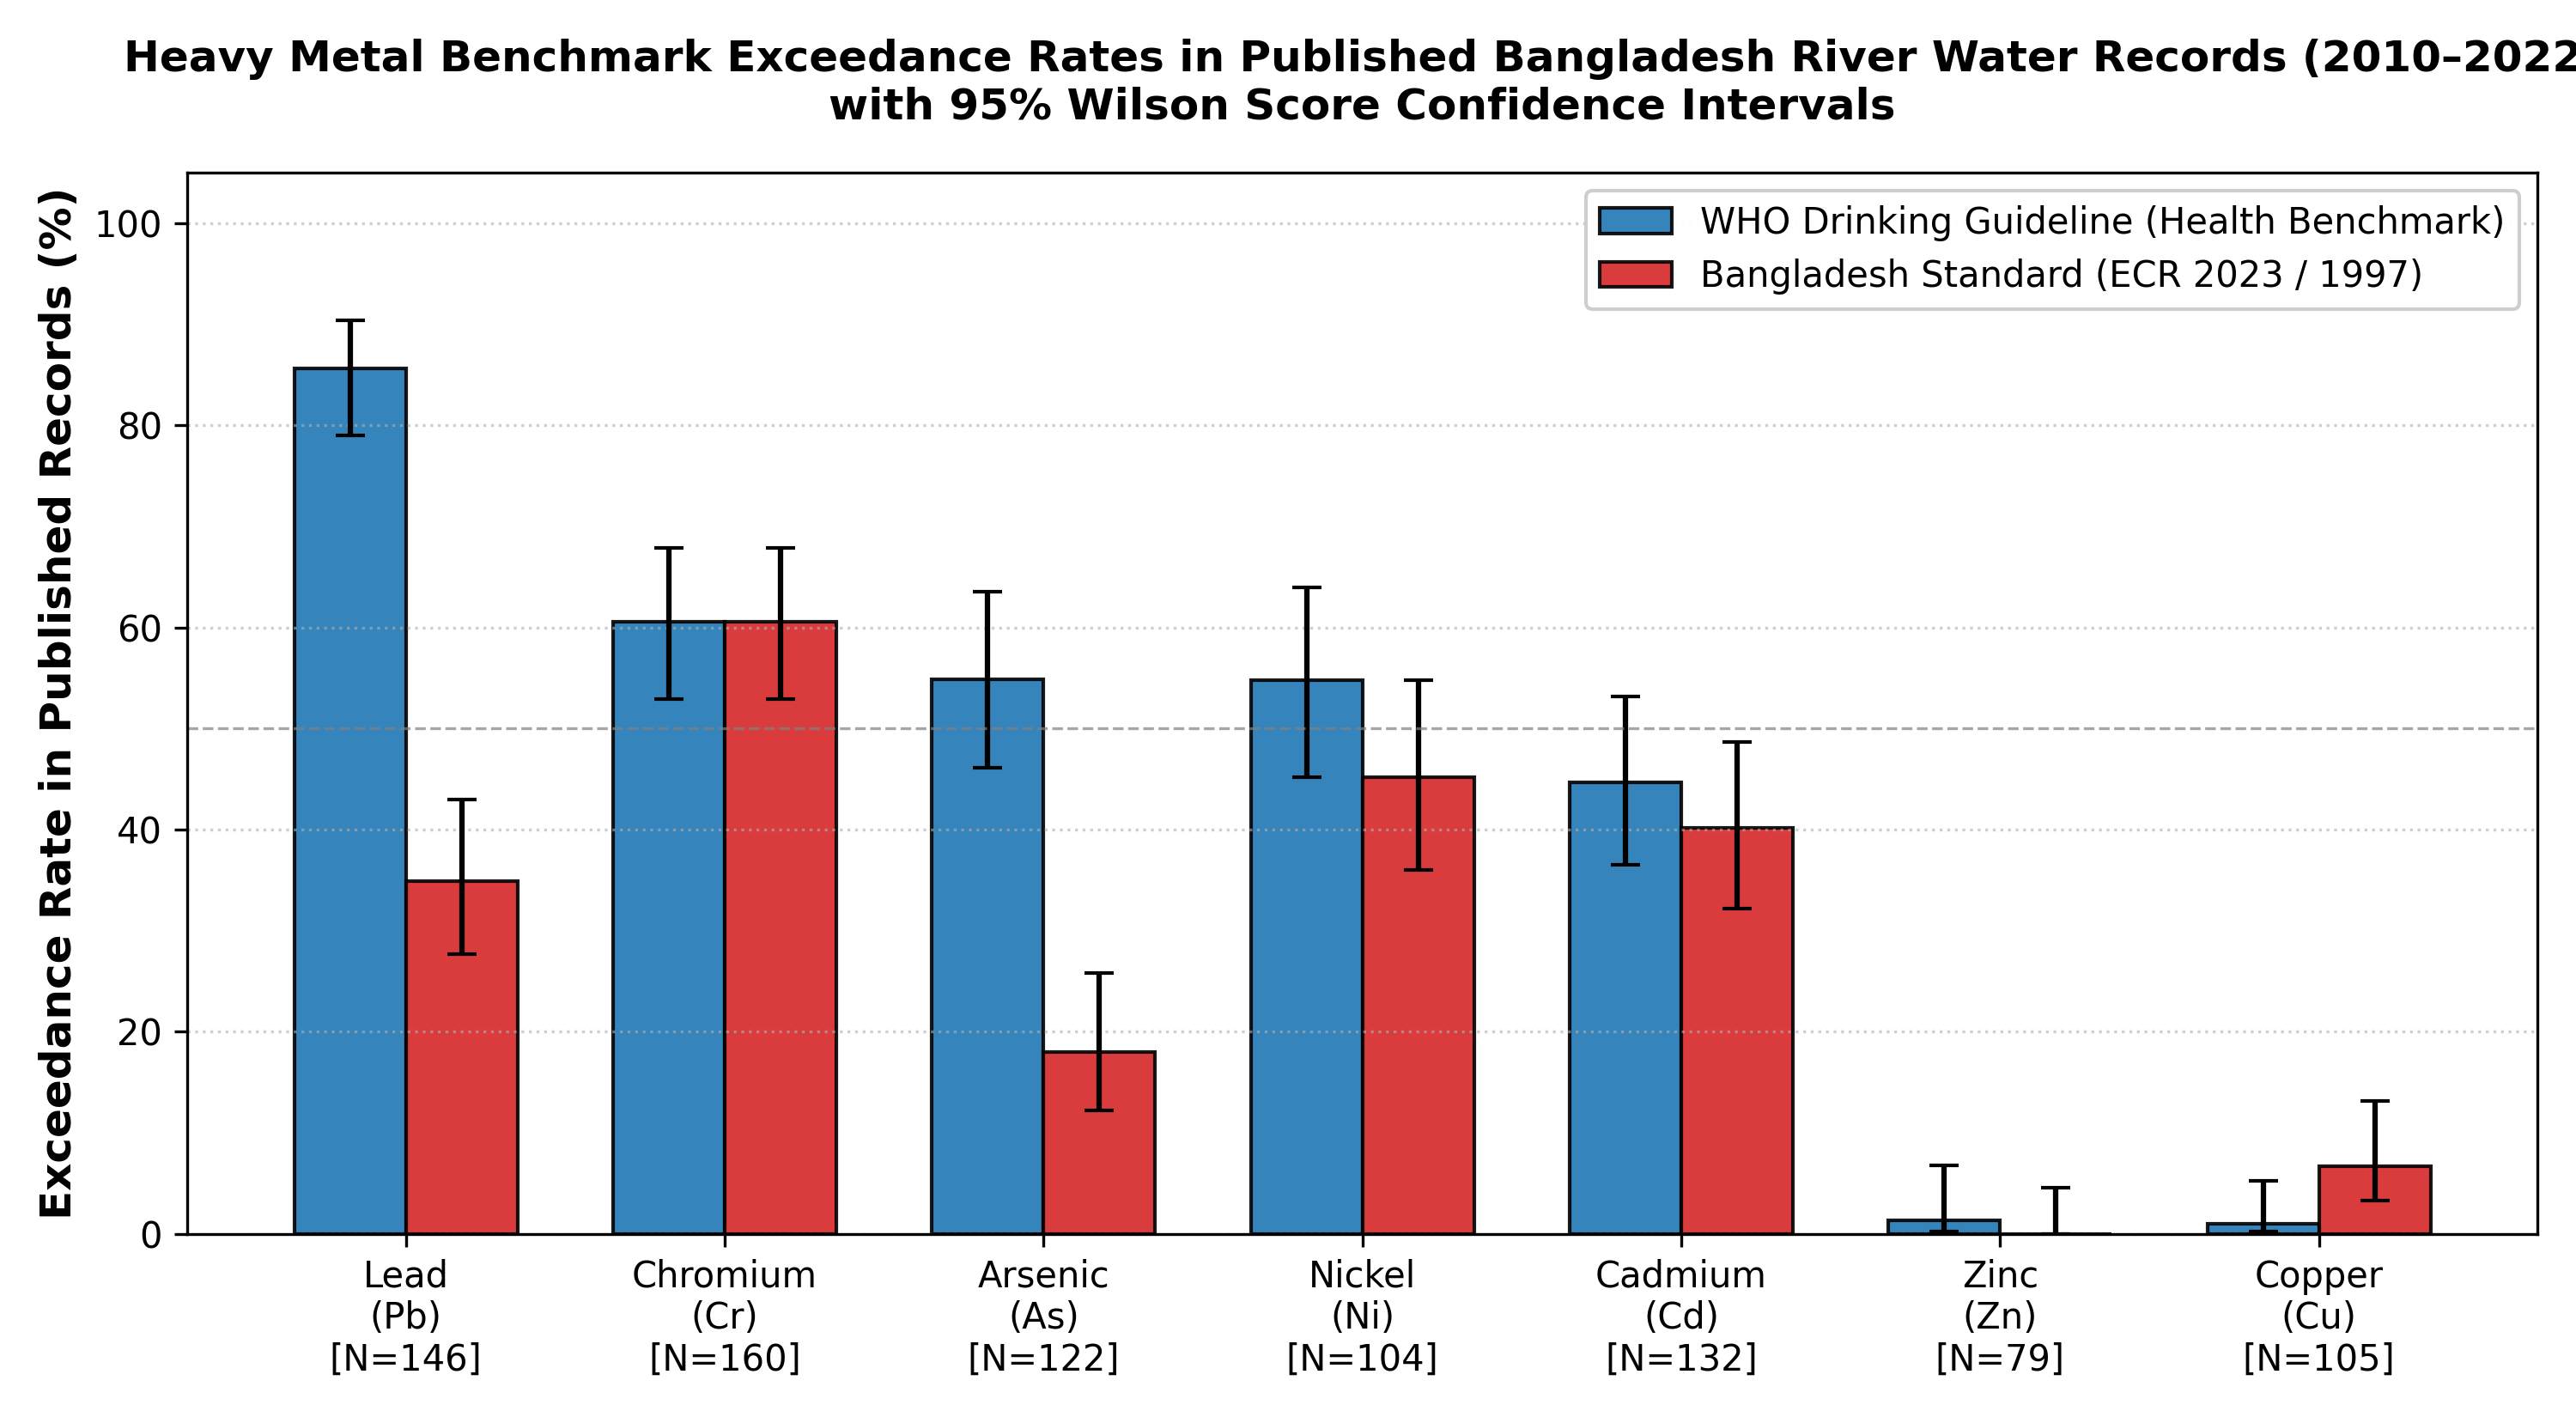
\includegraphics[width=0.92\textwidth]{fig1_exceedance.png}
\caption{Benchmark exceedance rates of dissolved and unspecified-fraction heavy metals across published Bangladesh river water records (2010--2022) with 95\% Wilson score confidence intervals.}
\label{fig:exceedance}
\end{figure}

\subsection{Integrated Multi-Metal Pollution Indices ($\mathrm{HPI}$, $\mathrm{HEI}$, $\mathrm{MI}$)}
Evaluation of composite multi-metal indices across 157 records showed elevated cumulative loadings (Table~\ref{tab:indices}):
\begin{itemize}
    \item \textbf{Heavy Metal Pollution Index ($\mathrm{HPI}$):} Across all multi-metal records, the median $\mathrm{HPI}$ was \textbf{202.30} (IQR: 79.01--793.90), with a mean of 718.74 and maximum of 5,920.11. Overall, \textbf{63.1\%} of records (99/157) exceeded the critical threshold of 100, and \textbf{50.3\%} (79/157) fell into the high contamination category ($\mathrm{HPI} > 200$).
    \item \textbf{River-Specific Variations:} High median $\mathrm{HPI}$ values were documented in the Meghna (median: 2,155.33), Buriganga (median: 1,839.81), Shitalakhya (median: 793.90), and Padma (median: 524.86). In contrast, the southern coastal rivers Kirtankhola (median: 57.06) and Rupsa (median: 51.35) maintained median $\mathrm{HPI} < 100$, reflecting lower industrial metal loadings.
    \item \textbf{$\mathrm{HEI}$ and $\mathrm{MI}$ Results:} The median $\mathrm{HEI}$ was 8.21 (mean: 23.77), and the median $\mathrm{MI}$ was 3.83 (mean: 13.11), corroborating the spatial distribution identified by $\mathrm{HPI}$.
\end{itemize}

\begin{table}[htbp]
\centering
\small
\caption{Multi-metal pollution indices ($\mathrm{HPI}$, $\mathrm{HEI}$, $\mathrm{MI}$) synthesized across Bangladesh river systems.}
\label{tab:indices}
\begin{adjustbox}{width=\textwidth,center}
\begin{tabular}{lcccccccc}
\toprule
River System & $N$ & Mean $\mathrm{HPI}$ & Median $\mathrm{HPI}$ & IQR $\mathrm{HPI}$ & $\%\, \mathrm{HPI} > 100$ & $\%\, \mathrm{HPI} > 200$ & Median $\mathrm{HEI}$ & Median $\mathrm{MI}$ \\
\midrule
\textbf{Meghna} & 3 & 2,118.62 & 2,155.33 & 432.01 & 100.0\% & 100.0\% & 47.53 & 22.13 \\
\textbf{Buriganga} & 31 & 1,797.74 & 1,839.81 & 1,302.34 & 90.3\% & 90.3\% & 53.87 & 25.62 \\
\textbf{Shitalakhya} & 3 & 1,080.80 & 793.90 & 714.94 & 100.0\% & 100.0\% & 44.79 & 20.32 \\
\textbf{Padma} & 6 & 679.34 & 524.86 & 1,304.99 & 50.0\% & 50.0\% & 11.00 & 2.66 \\
\textbf{Karnaphuli} & 24 & 269.43 & 232.14 & 133.47 & 95.8\% & 66.7\% & 8.15 & 4.00 \\
\textbf{Korotoa} & 40 & 317.04 & 194.68 & 327.31 & 77.5\% & 50.0\% & 11.08 & 4.79 \\
\textbf{Turag} & 13 & 1,704.05 & 172.36 & 3,337.68 & 61.5\% & 46.2\% & 4.99 & 4.29 \\
\textbf{Kirtankhola} & 30 & 60.21 & 57.06 & 42.05 & 0.0\% & 0.0\% & 3.22 & 1.31 \\
\textbf{Rupsa} & 7 & 47.28 & 51.35 & 9.47 & 0.0\% & 0.0\% & 2.06 & 0.78 \\
\midrule
\textbf{All Multi-Metal Records} & 157 & 718.74 & \textbf{202.30} & 714.89 & \textbf{63.1\%} & \textbf{50.3\%} & 8.21 & 3.83 \\
\bottomrule
\end{tabular}
\end{adjustbox}
\end{table}

\subsection{Seasonal Dilution Dynamics}
Two-sided Mann-Whitney U hypothesis testing confirmed element-specific seasonal patterns between the winter dry season and the monsoon wet season (Table~\ref{tab:dilution}, Fig.~\ref{fig:dilution}).

\begin{table}[htbp]
\centering
\small
\caption{Seasonal comparison of heavy metal concentrations in Bangladesh rivers (Dry/Winter vs.\ Wet/Rainy season) with two-sided Mann-Whitney U tests and Holm-Bonferroni adjusted $p$-values.}
\label{tab:dilution}
\begin{adjustbox}{width=\textwidth,center}
\begin{tabular}{lcccccccc}
\toprule
Element & Dry $N$ & Dry Med (mg/L) & Wet $N$ & Wet Med (mg/L) & Ratio & Mann-Whitney $U$ & Two-Sided $p$ & Holm $p_{\mathrm{adj}}$ \\
\midrule
\textbf{Arsenic (As)} & 57 & 0.0073 & 23 & 0.0042 & \textbf{1.74$\times$} & 927.5 & \textbf{0.0039} & \textbf{0.0273$^*$} \\
\textbf{Chromium (Cr)} & 73 & 0.0710 & 28 & 0.0354 & 2.01$\times$ & 1,312.0 & 0.0281 & 0.1684 \\
\textbf{Cadmium (Cd)} & 59 & 0.0015 & 27 & 0.0008 & 1.88$\times$ & 1,014.5 & 0.0429 & 0.2147 \\
\textbf{Zinc (Zn)} & 27 & 0.5300 & 17 & 0.0725 & 7.31$\times$ & 300.0 & 0.0915 & 0.3661 \\
\textbf{Copper (Cu)} & 40 & 0.0866 & 16 & 0.0571 & 1.52$\times$ & 391.0 & 0.2009 & 0.6027 \\
\textbf{Nickel (Ni)} & 40 & 0.0685 & 18 & 0.0945 & 0.73$\times$ & 376.5 & 0.7880 & 1.0000 \\
\textbf{Lead (Pb)} & 67 & 0.0253 & 25 & 0.0287 & 0.88$\times$ & 859.0 & 0.8538 & 1.0000 \\
\bottomrule
\multicolumn{9}{l}{\footnotesize $^*$Statistically significant after Holm-Bonferroni family-wise error rate adjustment ($\alpha = 0.05$).}
\end{tabular}
\end{adjustbox}
\end{table}

Key findings:
\begin{itemize}
    \item \textbf{Significant Seasonal Dilution for Arsenic:} Arsenic demonstrated a statistically significant seasonal contrast, with dry-season median concentrations 1.74 times higher than wet-season concentrations (0.0073 vs.\ 0.0042~mg/L; two-sided $p = 0.0039$, Holm-adjusted $p_{\mathrm{adj}} = 0.0273$).
    \item \textbf{Unadjusted Trends for Chromium and Cadmium:} Chromium (dry median 0.0710 vs.\ wet 0.0354~mg/L; ratio 2.01$\times$, unadjusted $p=0.0281$) and Cadmium (dry median 0.0015 vs.\ wet 0.0008~mg/L; ratio 1.88$\times$, unadjusted $p=0.0429$) both displayed approximately two-fold higher dry-season medians. However, after applying Holm-Bonferroni correction for multiple hypothesis testing across the seven metals, neither relationship met the 0.05 significance threshold ($p_{\mathrm{adj}} = 0.168$ for Cr; $p_{\mathrm{adj}} = 0.215$ for Cd).
    \item \textbf{Absence of Seasonal Contrast for Lead and Nickel:} Lead (dry median 0.0253 vs.\ wet 0.0287~mg/L; ratio 0.88$\times$, $p=0.8538$) and Nickel (dry median 0.0685 vs.\ wet 0.0945~mg/L; ratio 0.73$\times$, $p=0.7880$) showed no significant dilution, with wet-season medians remaining slightly higher than dry-season medians.
\end{itemize}

\begin{figure}[htbp]
\centering
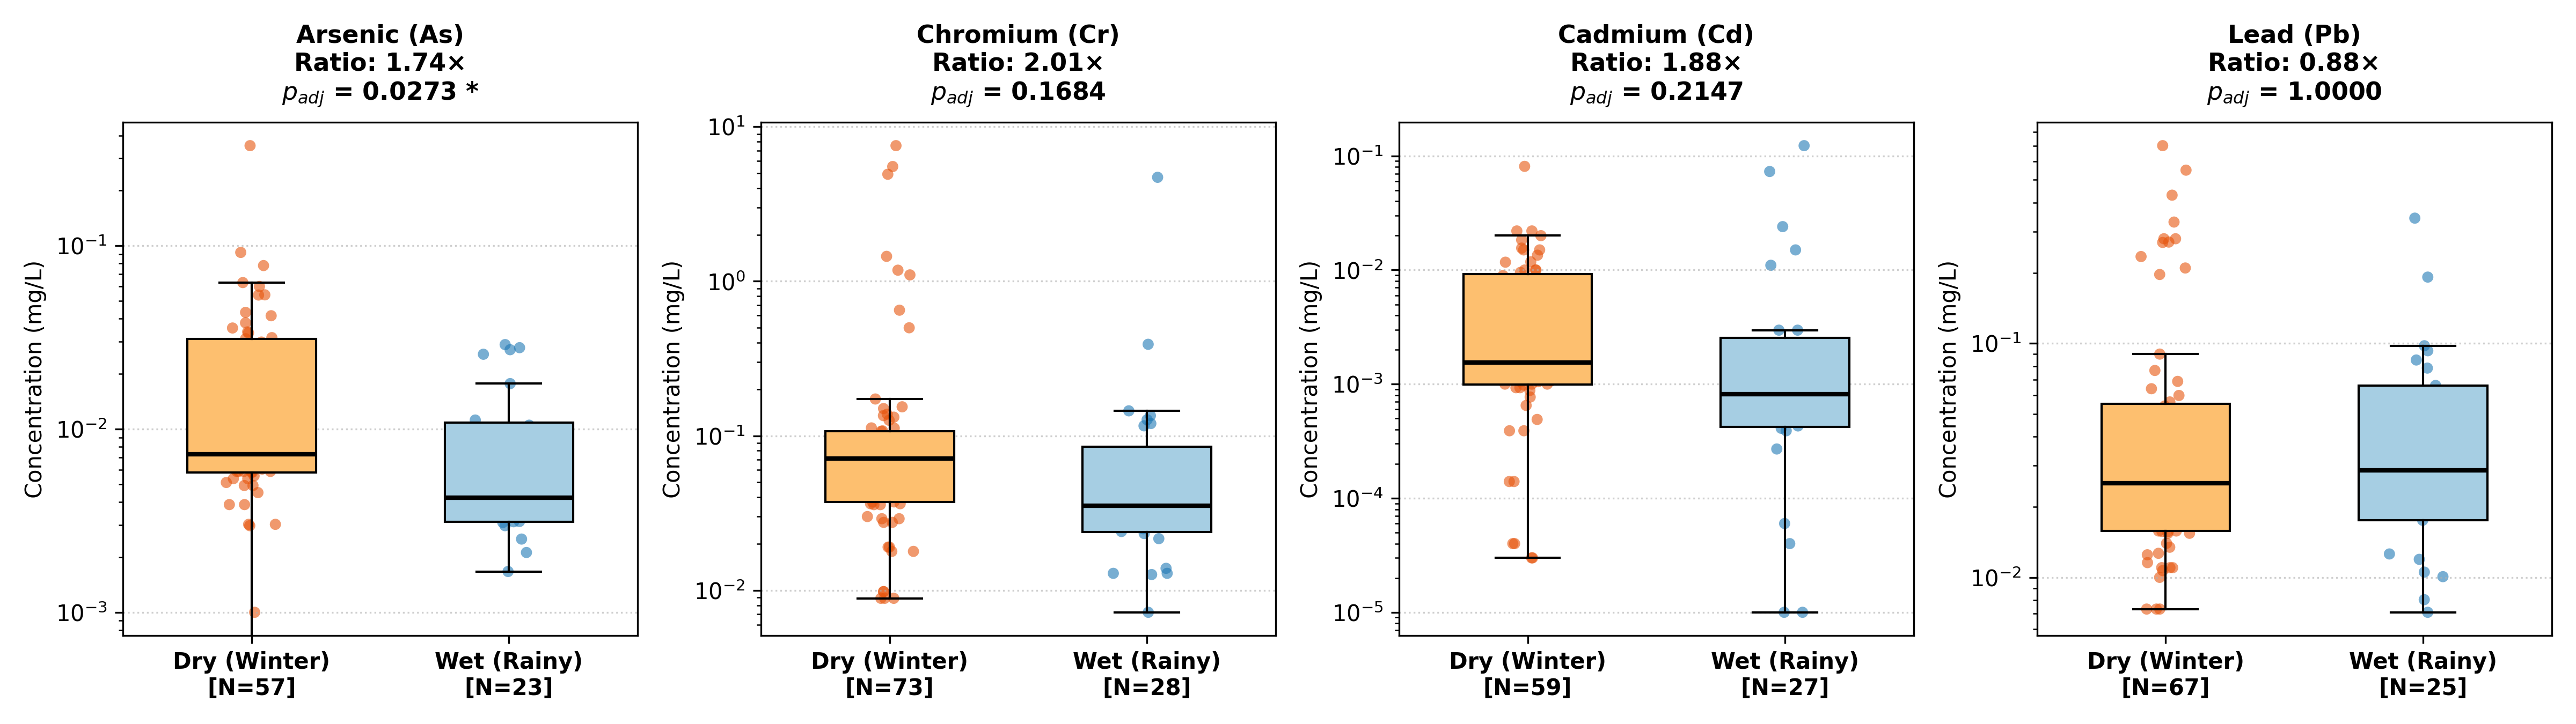
\includegraphics[width=0.98\textwidth]{fig2_dilution.png}
\caption{Log-scale seasonal distributions (Dry/Winter vs.\ Wet/Rainy) for Arsenic, Chromium, Cadmium, and Lead across Bangladesh rivers with individual observations overlayed.}
\label{fig:dilution}
\end{figure}

\subsection{Spatial Coverage and Geographic Surveillance Gaps}
Geodesic distance routing across HydroSHEDS HydroRIVERS revealed that current academic literature has left extensive portions of Bangladesh's primary river systems unstudied:
\begin{itemize}
    \item \textbf{Network-Wide Coverage Extent:} Out of 3,894 major river reach segments (Strahler order $\ge 4$, $Q \ge 50\text{ m}^3/\text{s}$) strictly within Bangladesh territory (totaling 8,369.5~km), \textbf{3,408 reaches (87.5\%, totaling 7,372.3~km)} are situated more than 25~km away from any published sampling point.
    \item \textbf{Multi-Threshold Analysis:} At a 10~km threshold, 96.1\% of major reach length (8,041.2~km) lacks coverage; at 50~km, 69.8\% of major reach length (5,844.7~km) remains unrepresented in published heavy metal literature.
    \item \textbf{Geographically Dispersed Surveillance Candidates:} Rather than clustering along a single channel, candidate reaches distributed across the major river systems were prioritized (Table~\ref{tab:stations}), spaced $\ge 30$~km apart across the Lower Meghna, Padma, Upper Ganges, and Jamuna/Brahmaputra mainstems.
\end{itemize}

\begin{table}[htbp]
\centering
\small
\caption{Prioritized candidate surveillance reaches across major Bangladesh river networks located $>25$~km from published monitoring points, enforcing $\ge 30$~km spatial separation.}
\label{tab:stations}
\begin{adjustbox}{width=\textwidth,center}
\begin{tabular}{clcccccl}
\toprule
Rank & Candidate ID & Lat ($^\circ$N) & Lon ($^\circ$E) & Order & Area ($\text{km}^2$) & $Q$ ($\text{m}^3/\text{s}$) & Target River Reach \\
\midrule
1 & \texttt{GAP\_STN\_01} & 23.227 & 90.631 & 9 & 1,574,223 & 40,393 & Lower Meghna Mainstem (Chandpur Confluence) \\
2 & \texttt{GAP\_STN\_02} & 23.395 & 90.395 & 9 & 1,488,391 & 34,906 & Padma-Meghna Convergence (Munshiganj Reach) \\
3 & \texttt{GAP\_STN\_03} & 23.535 & 90.144 & 9 & 1,485,761 & 34,854 & Lower Padma Main Channel (Madaripur) \\
4 & \texttt{GAP\_STN\_04} & 23.718 & 89.919 & 9 & 1,485,272 & 34,838 & Upper Padma Mainstem (Goalundo Reach) \\
5 & \texttt{GAP\_STN\_05} & 23.802 & 89.608 & 8 & 944,490 & 13,494 & Ganges-Jamuna Convergence Reach (Rajbari) \\
6 & \texttt{GAP\_STN\_06} & 23.919 & 89.309 & 8 & 943,786 & 13,479 & Upper Ganges Mainstem (Kushtia) \\
7 & \texttt{GAP\_STN\_07} & 24.200 & 88.750 & 8 & 942,749 & 13,507 & Central Ganges Channel (Pabna-Natore Reach) \\
8 & \texttt{GAP\_STN\_08} & 24.356 & 88.492 & 8 & 941,812 & 13,498 & North-West Padma Reach (Rajshahi Upstream) \\
9 & \texttt{GAP\_STN\_09} & 24.452 & 88.210 & 8 & 929,834 & 13,279 & Upper Border Ganges Reach (Chapai Nawabganj) \\
10 & \texttt{GAP\_STN\_10} & 24.089 & 89.695 & 8 & 521,878 & 20,698 & Lower Jamuna (Brahmaputra) Reach (Sirajganj) \\
11 & \texttt{GAP\_STN\_11} & 24.351 & 89.790 & 8 & 520,951 & 20,660 & Central Jamuna Mainstem (Bogra Reach) \\
12 & \texttt{GAP\_STN\_12} & 24.624 & 89.805 & 8 & 520,682 & 20,666 & Upper Jamuna Channel (Jamalpur-Bogra Reach) \\
13 & \texttt{GAP\_STN\_13} & 24.872 & 89.624 & 8 & 514,663 & 20,484 & Brahmaputra Confluence Reach (Gaibandha) \\
14 & \texttt{GAP\_STN\_14} & 25.146 & 89.694 & 8 & 514,278 & 20,833 & Upper Brahmaputra Channel (Kurigram) \\
15 & \texttt{GAP\_STN\_15} & 25.421 & 89.698 & 8 & 500,939 & 21,061 & Northern Brahmaputra Entry Reach (Chilmari) \\
\bottomrule
\end{tabular}
\end{adjustbox}
\end{table}

\section{Discussion}

\subsection{Benchmark Exceedances and Literature Selection Patterns}
Our multi-study synthesis demonstrates that trace metal concentrations reported in published studies frequently exceed conservative drinking water benchmarks. Specifically, Lead concentrations exceeded the WHO guideline of 0.010~mg/L in 85.6\% of records, with a median of 0.0286~mg/L and an audited maximum of 0.700~mg/L. Total Chromium (median: 0.0710~mg/L) and Nickel (median: 0.0888~mg/L) also exhibited widespread exceedances above international reference values.

However, interpreting these exceedance rates requires careful contextualization. As revealed by our sensitivity analysis, published data are disproportionately concentrated in rivers receiving intense industrial and municipal wastewater discharges from the Dhaka metropolitan area (Buriganga, Turag, Shitalakhya). When these rivers were removed, the national exceedance rate against Bangladesh statutory standards for Lead fell from 34.9\% to 18.3\%, and for Arsenic from 18.0\% to 8.9\%. This highlights that headline exceedance statistics reflect the focus of environmental researchers on known contamination hotspots rather than an unbiased census of all river water across Bangladesh.

\subsection{Potential Exposure Context and Health Implications}
Although these exceedances indicate substantial water quality degradation, direct potable consumption of raw surface water in Bangladesh is relatively uncommon because the majority of municipal and rural domestic water supply is derived from deep and shallow groundwater aquifers. Consequently, comparing untreated surface water with drinking water standards serves primarily as a comparative benchmark of chemical stress rather than a direct measure of potable exposure.

Nevertheless, elevated surface water concentrations remain ecologically and toxicologically relevant through secondary exposure pathways:
\begin{enumerate}
    \item \textbf{Agricultural Irrigation:} During the winter dry season, river water is heavily abstracted for boro rice cultivation and vegetable cropping. Long-term irrigation with metal-enriched water can elevate trace metal concentrations in agricultural topsoils and facilitate transfer into food crops \citep{Ali2021,Islam2015}.
    \item \textbf{Aquatic Bioaccumulation:} Dissolved and suspended trace metals are accumulated by benthic organisms and commercially harvested fish species \citep{Ahmad2010,Hossain2021,Mortuza2024}.
    \item \textbf{Direct Domestic Contact:} Riparian populations regularly use river water for bathing, washing, and livestock rearing, where dermal and incidental ingestion pathways remain relevant \citep{Saha2017}.
\end{enumerate}

Regarding elemental toxicity, we emphasize that analytical measurements reported in historical literature quantify \textbf{total Chromium} rather than distinguishing hexavalent $\mathrm{Cr(VI)}$ from trivalent $\mathrm{Cr(III)}$. While $\mathrm{Cr(VI)}$ is a confirmed human carcinogen, $\mathrm{Cr(III)}$ is significantly less toxic and is an essential micronutrient. Speciation-specific monitoring is required before precise toxicological risk can be assigned to observed Chromium loadings.

\subsection{Hydrological Mechanisms and Seasonal Dynamics}
The two-sided Mann-Whitney U test confirmed statistically significant seasonal dilution for Arsenic ($p = 0.0039$, $p_{\mathrm{adj}} = 0.0273$), with median concentrations declining from 0.0073~mg/L during the winter dry season to 0.0042~mg/L during the monsoon. Chromium and Cadmium exhibited similar two-fold dry-season median elevations, but did not maintain significance under Holm-Bonferroni correction.

The lack of seasonal dilution observed for Lead (dry median 0.0253 vs.\ wet median 0.0287~mg/L, ratio 0.88$\times$) and Nickel (ratio 0.73$\times$) indicates that monsoon hydrology involves contrasting solute mobilization mechanisms. During the dry season, low river discharge reduces volumetric dilution of continuous point-source industrial effluents. During the monsoon, while hydraulic discharge increases by orders of magnitude, intense precipitation can simultaneously mobilize diffuse non-point source contaminants from urban road surfaces, automotive maintenance yards, industrial scrap storage, and atmospheric depositions \citep{Li2018}. For elements associated with diffuse urban runoff such as Lead, increased non-point source wash-off during storm events may offset volumetric dilution from upstream discharge.

\subsection{Study Limitations}
Several inherent limitations of synthesizing published historical literature must be recognized:
\begin{enumerate}
    \item \textbf{Geographic and Publication Bias:} Published academic studies reflect convenience sampling directed at recognized pollution hotspots. As established in Section~3.4, over 87\% of major national river reach length lacks published heavy metal monitoring.
    \item \textbf{Fraction and Filtration Ambiguity:} Many published investigations did not state whether water samples underwent membrane filtration (e.g., 0.45~$\mu\text{m}$) or total acid digestion. Consequently, concentrations represent dissolved or unspecified fractions.
    \item \textbf{Analytical Heterogeneity:} Data were generated across 28 studies using different instrumentation (AAS, ICP-OES, ICP-MS), digestion chemistries ($\mathrm{HNO_3}$, aqua regia), and detection limits. Handling of values below detection limits was not uniformly documented in the source papers.
    \item \textbf{Confounding in Seasonal Analysis:} The seasonal comparison relies on pooling dry- and wet-season observations across different studies and river locations rather than multi-year repeated paired sampling at identical gauging stations. Variations in sampling year, river mix, and analytical methods between seasons introduce potential confounding.
    \item \textbf{Absence of Direct Exposure Assessment:} This study evaluates benchmark exceedance rather than conducting site-specific human exposure assessments (e.g., Target Hazard Quotients, Daily Intakes), because population water-intake rates and treatment data are not available across the synthesized literature.
\end{enumerate}

\section{Conclusions}
This study provides a comprehensive synthesis of published heavy metal data (2010--2022) across 12 major river systems in Bangladesh. Auditing 268 records against international and national drinking benchmarks revealed substantial exceedances: \textbf{85.6\%} of records exceeded the WHO drinking guideline for Lead (median: 0.0286~mg/L), and exceedances ranged from 44.7\% to 60.6\% for total Chromium, Nickel, Arsenic, and Cadmium. However, a sensitivity analysis excluding Greater Dhaka's peri-urban industrial rivers demonstrated that national exceedances are heavily influenced by hotspot clustering in academic literature. Integrated pollution indices classified 63.1\% of multi-metal records above the critical threshold ($\mathrm{HPI} > 100$, median: 202.30), with the highest contamination observed in the Meghna, Buriganga, and Shitalakhya rivers. Non-parametric hypothesis testing with family-wise Holm-Bonferroni correction confirmed statistically significant seasonal dilution for Arsenic (1.74$\times$ ratio, $p_{\mathrm{adj}} = 0.027$), while Lead and Nickel showed no seasonal dilution, suggesting compensatory non-point source urban wash-off during the monsoon. Finally, geodesic network routing in HydroSHEDS demonstrated that 87.5\% of major river reach length (7,372.3~km) remains unrepresented in published literature, providing 15 prioritized, geographically distributed candidate reaches to guide future surveillance deployments across the Lower Meghna, Padma, and Jamuna river basins.

\section*{CRediT Authorship Statement}
\textbf{Author 1:} Conceptualization, Formal Analysis, Methodology, Software, Writing -- Original Draft.
\textbf{Author 2:} Data Curation, Validation, Investigation, Resources.
\textbf{Author 3:} Supervision, Project Administration, Writing -- Review \& Editing.

\section*{Declaration of Competing Interest}
The authors declare that they have no known competing financial interests or personal relationships that could have appeared to influence the work reported in this paper.

\section*{Data Availability}
The curated dataset, reproducible analysis script, and GIS reach data are openly available in the repository at: \url{https://github.com/ShMazumder/heavy-metal.git}.

\bibliographystyle{elsarticle-harv}
\bibliography{references}

\end{document}
